\section{RRTCon  Class Reference}
\label{classRRTCon}\index{RRTCon@{RRTCon}}
Replaces Extend with Connect. 


{\tt \#include $<$rrt.h$>$}

Inheritance diagram for RRTCon::\begin{figure}[H]
\begin{center}
\leavevmode
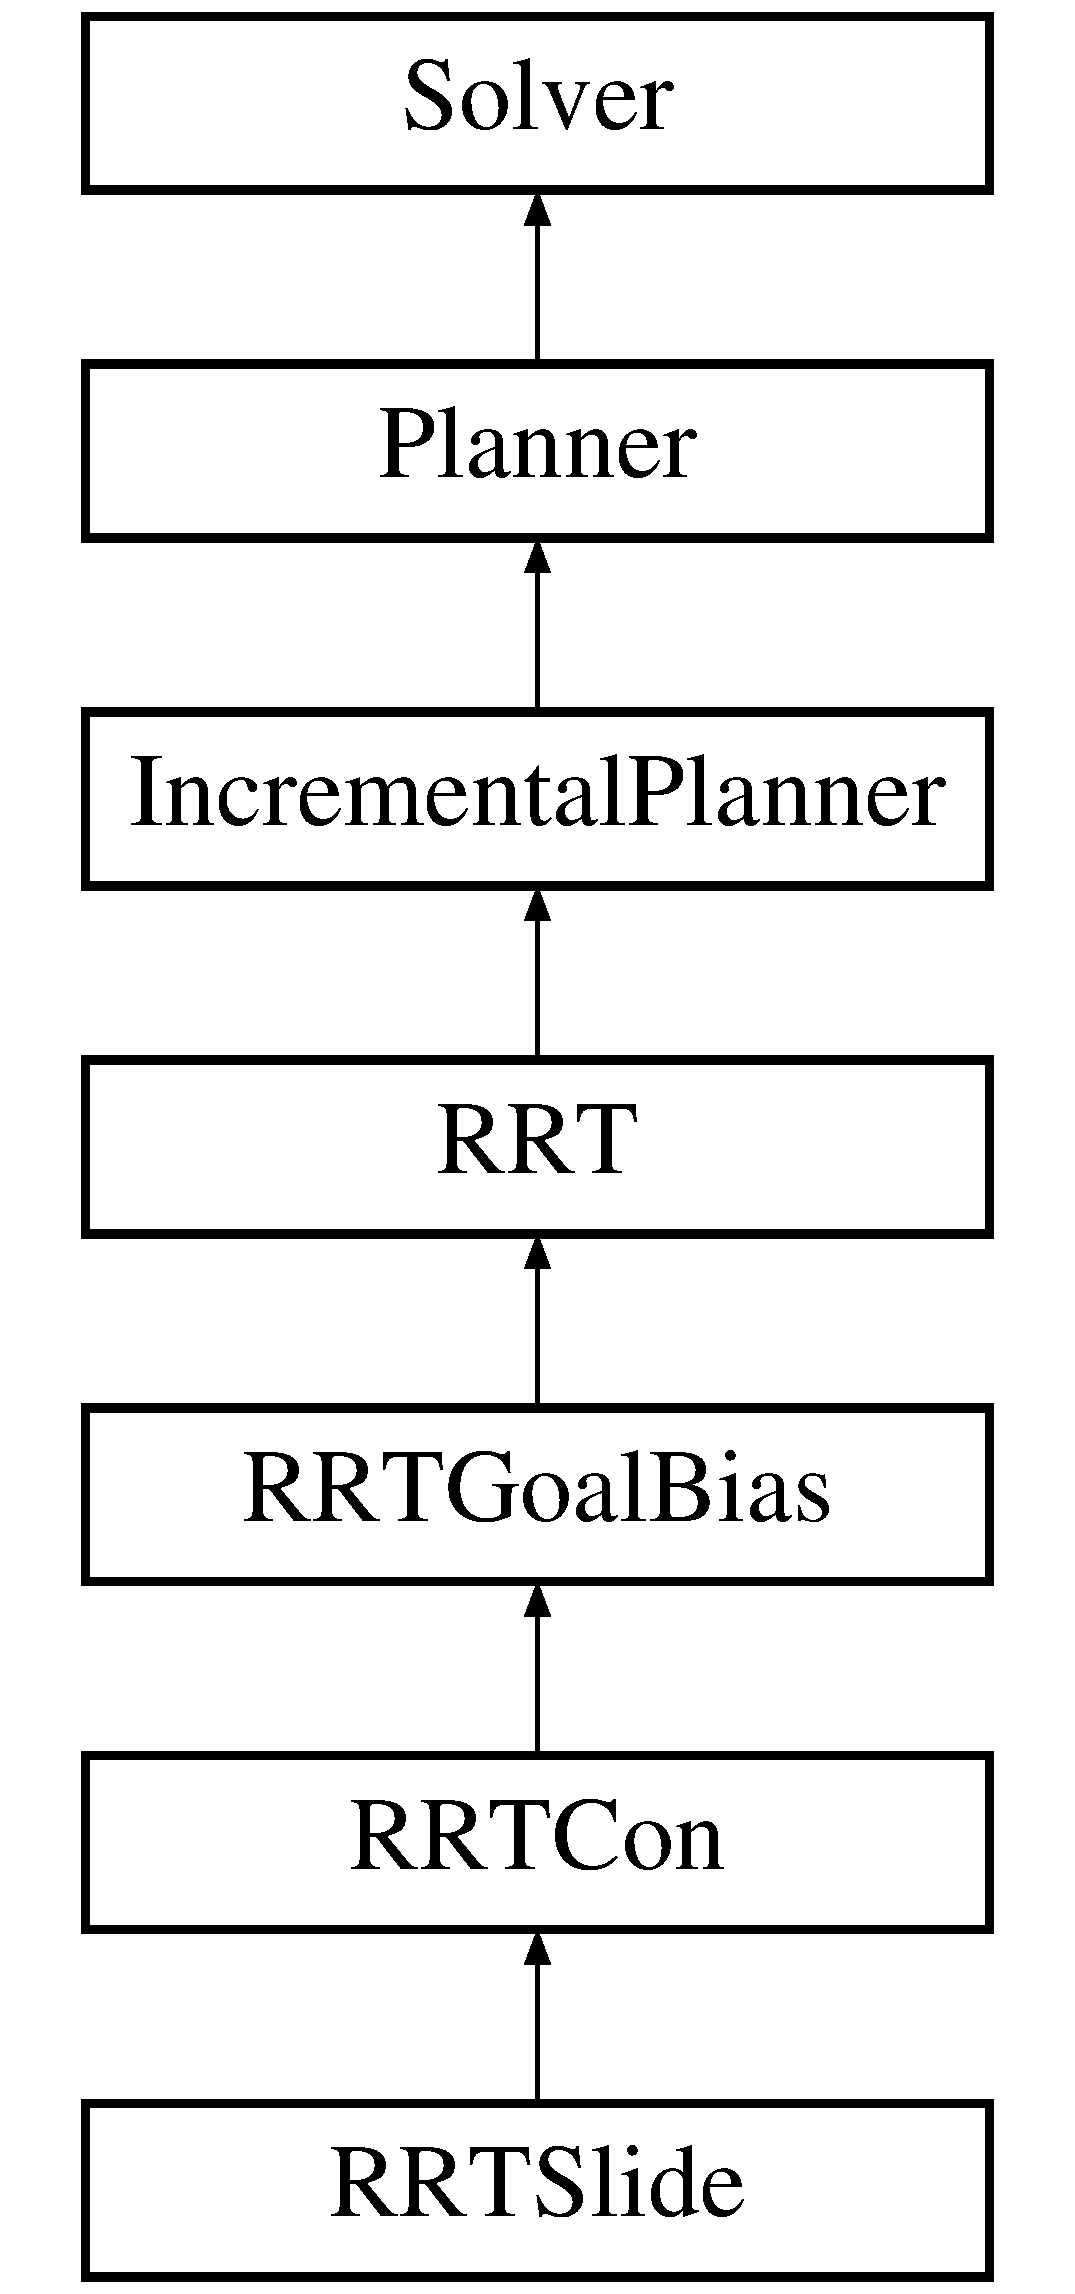
\includegraphics[height=7cm]{classRRTCon}
\end{center}
\end{figure}
\subsection*{Public Methods}
\begin{CompactItemize}
\item 
{\bf RRTCon} ({\bf Problem} $\ast$p)
\item 
virtual {\bf $\sim$RRTCon} ()
\begin{CompactList}\small\item\em An empty desctructor.\item\end{CompactList}\item 
virtual bool {\bf Plan} ()
\begin{CompactList}\small\item\em Here Extend is replaced by Connect. The tree is extended all the to the random sample, if possible.\item\end{CompactList}\end{CompactItemize}


\subsection{Detailed Description}
Replaces Extend with Connect.

The {\bf RRT} {\rm (p.\,\pageref{classRRT})} in the base class uses Extend to move a small amount in each step toward the random sample. In RRTCon, Extend is replaced by a method called Connect, which iterates the extension until the random sample is reached. Connect only adds the final  {\bf MSLNode} {\rm (p.\,\pageref{classMSLNode})} to the tree (not the intermediate increments). Since RRTCon is derived from {\bf RRTGoal\-Bias} {\rm (p.\,\pageref{classRRTGoalBias})}, a biasing probability can be set. By default, Goal\-Prob = 0.0. 



\subsection{Constructor \& Destructor Documentation}
\index{RRTCon@{RRTCon}!RRTCon@{RRTCon}}
\index{RRTCon@{RRTCon}!RRTCon@{RRTCon}}
\subsubsection{\setlength{\rightskip}{0pt plus 5cm}RRTCon::RRTCon ({\bf Problem} $\ast$ {\em p})}\label{classRRTCon_a0}


\index{RRTCon@{RRTCon}!~RRTCon@{$\sim$RRTCon}}
\index{~RRTCon@{$\sim$RRTCon}!RRTCon@{RRTCon}}
\subsubsection{\setlength{\rightskip}{0pt plus 5cm}virtual RRTCon::$\sim$RRTCon ()\hspace{0.3cm}{\tt  [inline, virtual]}}\label{classRRTCon_a1}


An empty desctructor.



\subsection{Member Function Documentation}
\index{RRTCon@{RRTCon}!Plan@{Plan}}
\index{Plan@{Plan}!RRTCon@{RRTCon}}
\subsubsection{\setlength{\rightskip}{0pt plus 5cm}bool RRTCon::Plan ()\hspace{0.3cm}{\tt  [virtual]}}\label{classRRTCon_a2}


Here Extend is replaced by Connect. The tree is extended all the to the random sample, if possible.



Reimplemented from {\bf RRT} {\rm (p.\,\pageref{classRRT_a3})}.

The documentation for this class was generated from the following files:\begin{CompactItemize}
\item 
{\bf rrt.h}\item 
{\bf rrt.C}\end{CompactItemize}
